\documentclass[twocolumn,letterpaper,10pt]{article}
\usepackage{times}
\usepackage{helvet}
\usepackage{courier}
\usepackage{txfonts}
\frenchspacing
%\setlength{\pdfpagewidth}{8.5in}
%\setlength{\pdfpageheight}{11in}

%used for pseudocode
\usepackage{algpseudocode}

%used to make charts
\usepackage{pgfplotstable}
\usepackage{pgfplots}

%used for mathematical notation
\usepackage{amsfonts}

%used to control spacing in table captions
\usepackage{subfig}

%used to import images
\usepackage{graphicx}

%used to specify table placement
\usepackage{float}

% Make it so lists don't have extra line spacing:
\usepackage{enumitem}
\setlist{noitemsep}

\usepackage{hyperref} % for \url

% For nice, customizable code listings:
\usepackage{listings}
\lstset{ %http://stackoverflow.com/questions/586572/make-code-in-latex-look-nice
	language=Java,
	basicstyle=\footnotesize,       % font size
	numbers=left,                      % where line numbers appear
	numberstyle=\footnotesize,   % size of line numbers
	stepnumber=1,                    % how often line numbers appear
	numbersep=5pt,                   % space between line numbers and code
	showstringspaces=false,       % whether or not to show a _ in strings
	frame=single,                       % what kind of frame should be around the code
	xleftmargin=1.5em,
	xrightmargin=1em,
	framexleftmargin=0em,
	%rulecolor=\color{black},         % for the frame
	tabsize=2,                             % set the number of spaces for tabs
	breaklines=true,                     % set whether or not linebreaking should occur
	breakatwhitespace=true,          % set whether or not linebreaking should occur only at spaces
	lineskip={-1.0pt}
	%commentstyle=\color{mygreen}, % color for code comments
	%numberstyle=\color{mygray}, % style for line numbers
}


\renewcommand{\today}{}

%\usepackage{plain} % for the bibliography

\title{Some Random Stuff in \LaTeX~to Serve as an Example}

\author{Some Author$^1$, Some Otherauthor$^2$, Steven Bogaerts$^1$ \\
\\
$^1$Department of Computer Science, DePauw University\\
Greencastle, IN 46135, U.S.A.\\
$^2$Department of Computer Science, Other Place College\\
Place, XY, 12345, U.S.A.\\
{\tt anonA@depauw.edu} \\
{\tt anonB@otherplace.edu} \\
{\tt stevenbogaerts@depauw.edu}
}

%define mathematical equations for repeated use
\newcommand{\sigmoid}{$$S(t)=\frac{1}{1+e^{-t}}$$}
\newcommand{\sigmoidprime}{$$S'(t)=S(t) \cdot (1 - S(t))$$}

\begin{document}

\maketitle

\begin{abstract}

This is where you write a quick summary that hopefully will get people interested in reading the entire paper.

\end{abstract}

\noindent {\bf Keywords:} keyword1, key phrase1, keyword2

\section{Introduction}

Throughout this document, I include snippets of a paper I wrote with some students years ago, about neural networks. You can ignore that actual text (I deleted a lot, so it won't make sense), and just focus on the \LaTeX~ideas. I left you lots of notes, in {\it italics}. For this document to be useful to read, make sure you're looking at both the .tex file and the generated pdf, at the same time. That way, you can see how the .tex code corresponds to what is actually in the paper. For example, peek at this paragraph in the .tex file now and note how I made some text italicized.

Please start by looking at all the stuff in the .tex file before the ``section Introduction'' part.  Big picture, it's loading in modules for various types of functionality. Then the part about setting the title, author information, and abstract is easy enough to figure out (just copy to another document if you're making a new paper). I recommend you take a ``I'll look into it if I need it'' attitude on the details of the code above.

Note that if you're submitting a paper to a particular venue (conference, journal, edited book), they'll often have a template document loading in what you need and setting things up according to their specifications. The template may also include separate files, like an .sty ``style file'' that customizes document processing.

You can skip to Section~\ref{sec:NN} in a moment. First, though, note how I referred to that section in the .tex file, and how that section is labeled. Don't hardcode section numbers!

Do you know about Lorem ipsum? This is just some filler text. You can skip to Section~\ref{sec:NN} now. Lorem ipsum dolor sit amet, consectetur adipiscing elit, sed do eiusmod tempor incididunt ut labore et dolore magna aliqua. Ut enim ad minim veniam, quis nostrud exercitation ullamco laboris nisi ut aliquip ex ea commodo consequat. Duis aute irure dolor in reprehenderit in voluptate velit esse cillum dolore eu fugiat nulla pariatur. Excepteur sint occaecat cupidatat non proident, sunt in culpa qui officia deserunt mollit anim id est laborum.

Sed ut perspiciatis unde omnis iste natus error sit voluptatem accusantium doloremque laudantium, totam rem aperiam, eaque ipsa quae ab illo inventore veritatis et quasi architecto beatae vitae dicta sunt explicabo. Nemo enim ipsam voluptatem quia voluptas sit aspernatur aut odit aut fugit, sed quia consequuntur magni dolores eos qui ratione voluptatem sequi nesciunt. Neque porro quisquam est, qui dolorem ipsum quia dolor sit amet, consectetur, adipisci velit, sed quia non numquam eius modi tempora incidunt ut labore et dolore magnam aliquam quaerat voluptatem. Ut enim ad minima veniam, quis nostrum exercitationem ullam corporis suscipit laboriosam, nisi ut aliquid ex ea commodi consequatur? Quis autem vel eum iure reprehenderit qui in ea voluptate velit esse quam nihil molestiae consequatur, vel illum qui dolorem eum fugiat quo voluptas nulla pariatur?

\section{Neural Networks}
\label{sec:NN}

\begin{figure}
\begin{center}
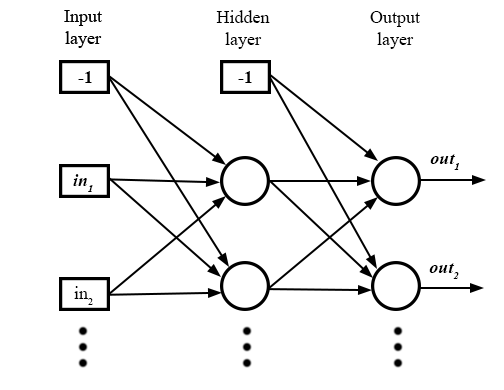
\includegraphics[width=.95\linewidth,height=2.5in]{neuralnetwork.png}
\end{center}
\caption{The structure of a simple neural network}
\label{fig:NN}
\end{figure}

{\it If you want to quote something, use two single backquotes (the key left of the 1) for the start, and two single quotes for the end: ``I'm quoting something correctly''. Don't do this: "I'm quoting something incorrectly" because it doesn't render the starting quotes correctly (subtle difference).}

A feed-forward neural network \cite{AImodern} maps a set of inputs... {\it Did you see that citation, there? More on citations soon.} Figure~\ref{fig:NN} shows a feed-forward neural network with a single hidden layer. {\it See how to refer to a figure? Don't hardcode the numbers! Also note the code to include a figure, starting with the begin figure command... I never memorize that. I've just been copying from one document to another all my life, figuring out how to make small adjustments via Google as needed. You have to make sure you have a corresponding file, though, like neuralnetwork.png. It's easiest to stick wtih .png files, though there are ways to render other graphics files if you need to look it up sometime.}

{\it Also note that Figure~\ref{fig:NN} ``floats''. That is, it doesn't automatically show up precisely where you put the code for it. \LaTeX~determines a good placement. If you don't like how it's placed, there are things you can do to force it to be elsewhere.}

Each unit's output is computed based on its inputs as follows: 

$$
out_k = S\left( \sum_{i=1}^n W_{ik}in_{i} \right)
$$
where $n$ is the number of inputs to node $k$, $W_{ik}$ is the weight from input $i$ to node $k$, $in_{i}$ is the input from i, 

{\it Double dollar signs around some ``MathJax'' code puts some math on a line by itself. Single dollar signs makes it ``inline''. Underscore is for subscript, caret for superscript. Notice the commands for left and right parenthesis (automatically sized), and sum.}

{\it Use braces for superscripts and subscripts that are more than one letter. Do this: $x_{ij}$, not this: $x_ij$.}

and S is the sigmoid function:
\sigmoid

{\it I needed to refer to sigmoid so much that I made a command for it. Do a find on ``newcommand'' at the top of the file to see how.}

{\it Study these MathJax examples! You'll want to write your own equations soon.}

The learning rate and momentum are both used in the weight update rules that follow. For the hidden-output weights:
$$\Delta W_{ji} = \alpha \cdot Err_i \cdot S'(in_i) \cdot x_j + \mu(old\Delta W_{ji})$$
such that
$$in_i = \sum_{j = 1}^n W_{ji}x_j$$
$$Err_i = f_i(\vec{x}) - S(in_i)$$
For input-hidden weights:
$$\Delta W_{kj} = \alpha \cdot x_k \cdot \Delta_j$$
such that
$$\Delta_j = S'(in_j) \cdot \sum_{i} W_{ji} \cdot \Delta_i$$
$$\Delta_i = Err_i \cdot S'(in_i)$$
where $k$ is an input unit index, $j$ is a hidden unit index, $i$ is an output unit index, $f$ is the target function (so $f_i(\vec{x})$ is the activation of output unit $i$ in the known example with inputs $\vec{x}$), $x_k$ and $x_j$ refer to the activation of input and hidden units respectively, $\alpha$ is the learning rate, $\mu$ is the momentum, $W_{xy}$ is the weight from node $x$ to node $y$, $n$ is the number of hidden units, $old\Delta W_{ji}$ is the change made to the weight in the previous update, and $S'$ is the derivative of the sigmoid function:

$$S'(t) = S(t) \cdot (1-S(t))$$

{\it For more examples of MathJax, check out the math.tex and corresponding math.pdf files. Then also look at symbols.pdf. Be familiar with generally what's in these documents, so you can look up information as needed. Google will help for this too, of course.}

\section{Experiments}
\subsection{Setup}
Stuff here

\subsubsection{Lots of subs!}
Indeed. Three subs requires some special library, though.

You can make bulleted lists:
\begin{itemize}
	\item Itemized lists
	\item Enumerated lists
\end{itemize}

\noindent and enumerated lists:
\begin{enumerate}
	\item Itemized lists
	\item Enumerated lists
\end{enumerate}

%\subsubsubsection{Error!}

{\it Hey, I commented out a line using the percent sign. So how can I make a percent sign show up in my document? I ``escape'' it with a backslash. It works 100\% of the time. However, if you forget to escape it and write 100% then it comments out this part of your text!
}

\section{Results}

\subsection{Cars Data Set Results}

\begin{figure}
\begin{center}
\begin{tikzpicture}
\begin{axis}[width=.95\linewidth,
	xlabel=Number of Epochs,
	ylabel=Average Error, 
	axis lines=left,
	xtick={100, 500, 1000},
	xmin=0, xmax=1100,
	ytick={0.02, 0.04, 0.06, 0.08, 0.1},
	ymin=0,
	scaled y ticks = false,
	y tick label style={/pgf/number format/fixed}]
\addplot [only marks, mark size=1pt] table[y=$avg_err$, x=num_epochs]{carsnumepochs.dat};
\end{axis}
\end{tikzpicture}
\end{center}
\caption{Cars: Effect of the number of epochs on average error.}
\label{fig:CarsNumEpochs}
\end{figure}

Figure \ref{fig:CarsNumEpochs} shows that.... {\it Note how I generated the graph in the document itself, reading from a .dat file. Usually I just make the graph in Excel or something and load it in as an image, but now you know this is possible too.}

{\it Here's a tip, if you're grabbing an image from Excel: Zoom in as much as you can, so that the image is massive, filling up the screen. Then take a screenshot. The image will be too big, but you can reduce its size. The purpose of taking a screenshot all zoomed in is so that the screenshot is a higher resolution. I do this all the time; it makes a big difference.}

{\it For screenshots, personally, I like the free tool Cropper at \url{https://archive.codeplex.com/?p=cropper}. Did you notice just above how that URL is a link? Note how to do that.}

\begin{table}
\caption{Cars: Amount of results settled below 50\% of maximum batch size.}
\label{tbl:CarsBatchSize}
\centering
\begin{tabular}{c c c}
\hline
Max Batch Size & Experiments Run & $<50\%$ of Max \\
\hline
50 & 54 & 40 \\
100 & 17 & 17 \\
150 & 8 & 7 \\
\hline
\end{tabular}
\end{table}

When examining batch size, .... Table~\ref{tbl:CarsBatchSize} summarizes these results. {\it Note the code for generating and referring to a table. This is a floating table, like we had a floating image before. There's a super handy tool for making a table online: \url{https://www.tablesgenerator.com/}. Try it out a bit.}

\section{Code}

{\it Generally it's not appropriate to put a ton of code in your paper, but some can be useful in some circumstances. It's probably best to put it in a figure, like Figures~\ref{fig:ols} and~\ref{fig:adderManager}.}

\begin{figure}
	\begin{center}
		\begin{algorithmic}
			\State {\bf Ordinary Least Squares}
			\State {\bf INPUT} ($X = \{\vec{x}^{(i)}\}$, $Y = \{y^{(i)}\}$, $\alpha$)
			\State \Comment{There are $n$ data elements, each with $m$ independent variable values. That is, $i \in \mathbb{Z}$, $1 \leq i \leq n$, and $\forall i, \vec{x}^{(i)}$ has $m$ elements.}
			\State {\bf OUTPUT} $\vec{\theta}$
			\State $\vec{\theta} \leftarrow$ arbitrary initial values
			\Repeat
			\For{$i = 1, n$} \Comment For each data element $(\vec{x}^{(i)}, y^{(i)})$
			\State $x_0^{(i)} \leftarrow 1$ \Comment To update $\theta_0$
			\For{$j = 0, m$} \Comment For each model parameter $\theta_j$
			\State $t_j \leftarrow \theta_j - \alpha x_j^{(i)} (h_{\vec{\theta}}(\vec{x}^{(i)}) - y^{(i)})$
			\EndFor
			\State $\vec{\theta} \leftarrow \vec{t}$ \Comment Batch update
			\EndFor
			\Until{change in $\vec{\theta}$ is below some threshold}
			\State {\bf return} $\vec{\theta}$
		\end{algorithmic}
	\end{center}
	\caption{Pseudocode for a batch-update iterative ordinary least squares process.}
	\label{fig:ols}
\end{figure}

\begin{figure}[t]
	\begin{lstlisting}
public void runExperiment() {
	int totalNums = 10000;
	int[] arr = makeRandomArray(totalNums);
	
	parallelSum = 0;
	PartialAdder add1 = new PartialAdder(this, arr, 0, totalNums/2);
	PartialAdder add2 = new PartialAdder(this, arr, totalNums/2, totalNums);
	add1.start();
	add2.start();
	add1.join();
	add2.join();
	System.out.println("In parallel, sum: " + parallelSum);
	
	int sequentialSum = computeSequentialSum(arr);
	System.out.println("Sequentially, sum: " + sequentialSum);
}
	
public void receiveMessage(int partialSum) {
	parallelSum += partialSum;
}
	\end{lstlisting}
	\caption{This method, in the {\tt AdderManager} class, spawns two child threads to sum the numbers in an array, and then reports their results.} \label{fig:adderManager}
\end{figure}

\section{Related Work}

{\it Just more citation examples here!}

The parallelization of neural networks has been the focus of much research. For example, \cite{Kim} describes... \cite{Gruau} describes a genetic algorithm... Another example of a genetic algorithm applied to neural networks can be found in \cite{Soares}.

{\it How can you include citations? There are a few steps. First, check out the end of this document. The line bibliography\{latexIntro\} means that the bibliography for this document is in the file called latexIntro.bib. Open up that document now, in a programming text editor like Notepad++ or Sublime. Observe the different ways to specify a document, based on its type and what information you have about it. So the bib file gives the data on the bibliography, and the way it actually shows up is determined by the bibliographystyle\{plain\} line at the end of your .tex file. 

Note in the .bib file that the first entry is called ``Bache''. So you can cite it like this: \cite{Bache} (note how this is done in the .tex file).

How can you learn the format for a .bib entry? Actually, you usually don't need to. Go to \url{scholar.google.com}. Search for something, for example ``gradient boosting regressor''. Suppose you read one document in the results and decide you want to cite it. Click the little quotes icon (just to the right of the star icon) for that entry. In the pop-up window, click ``BibTeX''. Copy what you see into your .bib file. Cool, huh?

If you need to cite a website, follow the example in latexIntro.bib, for the Bache entry.}

\section{Future Work}

Win the Super Bowl.

{\it There's a little extra spacing around these sections because \LaTeX~has decided there's not enough room to start the ``References'' section on this page.}

\section{Conclusion}
\LaTeX~has a bit of a learning curve, but you'll work it out, and then it's incredibly powerful.

\section{Acknowledgment}
Should be included if work is funded by some organization (e.g. the NSF), or there's just someone you want to thank for their professional contribution.

\bibliographystyle{plain}
\bibliography{latexIntro}

\end{document}
